\section{Interpretation of Results}\label{sec:interpretation}

The interpretation section will cover two main parts. 
Initially, we will display the effects of fixed costs and irreversibility by keeping $\gamma_{adj}$ constant at 2.0.
Subsequently, we will estimate a complete set of parameters, including $\gamma_{adj}$ and explore the outputs.

\vspace{\baselineskip}

\begin{figure}[H]
    \centering
    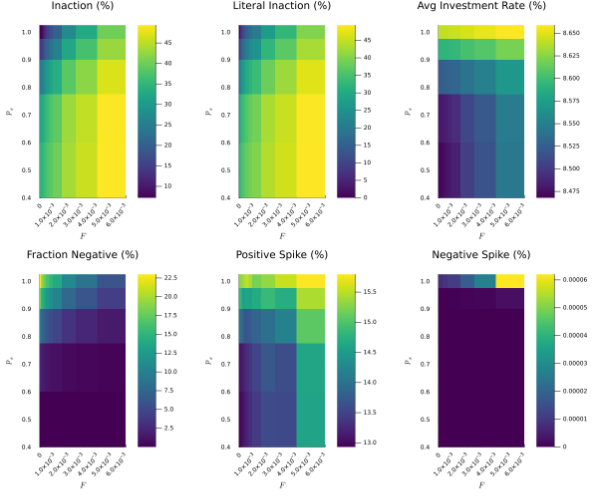
\includegraphics[width=0.8\textwidth]{fig/f_ps_moment_heatmap.png}
    \caption{Moments over a grid of $\{F, \rho_s\}$ combinations.}
    \label{fig:moment_heatmap}
\end{figure}

Figure~\ref{fig:moment_heatmap} computes the moments included in LRD and an additional metric \enquote{Literal Inaction}.
While \enquote{Inaction} includes small adjustments ($< 1\%$ of capital), \enquote{Literal Inaction} refers to the choice of inaction itself.

\vspace{\baselineskip}

Intuitively, inaction should increase with both fixed costs and irreversibility, which we observe in the moments.
Similarly, positive investment spikes follow an intuitive pattern, increasing with fixed costs and is relatively constant with respect to irreversibility.
Notably, we observe no negative investment spikes in the data where $\rho_s \neq 1.0$ and both spikes of both signs tend to increase with fixed costs.

\subsection{Case 1: Convex Costs}\label{subsec:convex_costs}
Case 1 depicts complete absence of fixed costs and irreversibility, which results in a convex adjustment cost function.
The expected result in this case would be adjustments in all periods. With no consequences for adjusting, the firm would always choose to adjust capital to the optimal level.

\vspace{\baselineskip}
\begin{minipage}{0.45\textwidth}
    \begin{figure}[H]    
        \centering
        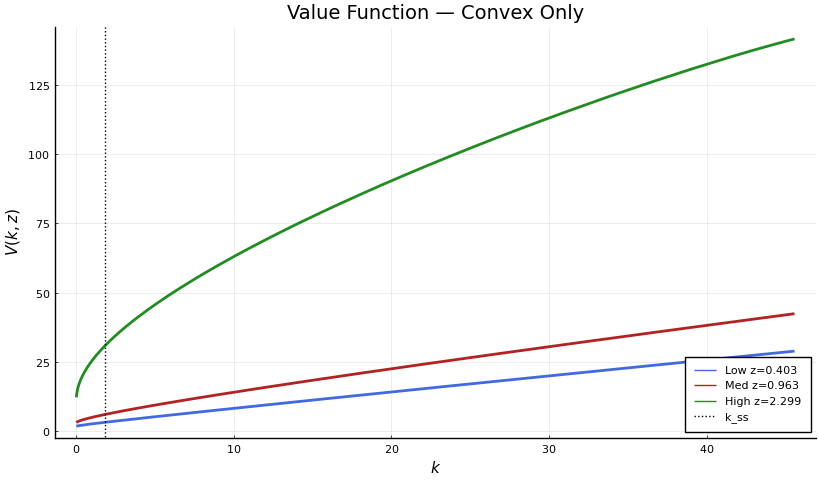
\includegraphics[width=0.8\textwidth]{fig/s1_value.png}
        \caption{Value Function for $z$ levels in Case 1}
        \label{fig:s1_value}
    \end{figure}
\end{minipage}\hfill
\begin{minipage}{0.45\textwidth}
    \begin{figure}[H]
        \centering
        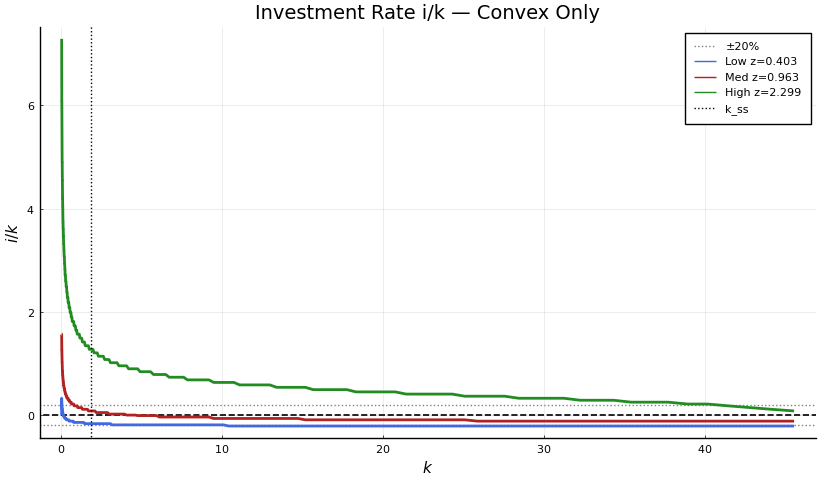
\includegraphics[width=0.8\textwidth]{fig/s1_ir.png}
        \caption{Investment Rates for $z$ levels in Case 1}
        \label{fig:s1_ir}
    \end{figure}
\end{minipage}

\vspace{\baselineskip}

Figure~\ref{fig:s1_value} depicts the value function at varying levels of productivity $z$.
We observe a smooth function and an increase in slope for higher $z$ levels, which is consistent with the intuition that higher productivity should lead to higher returns on capital and thus a steeper value function.
Investment rates in Figure~\ref{fig:s1_ir} show that high productivity firms never choose to disinvest while both low and medium productivity firms monotonically stay below 0 investment rates from a relatively early point.

\vspace{\baselineskip}
\begin{minipage}{0.45\textwidth}
    \begin{figure}[H]
        \centering
        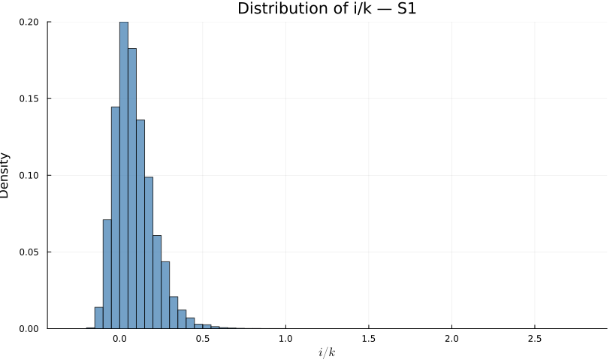
\includegraphics[width=\textwidth]{fig/s1_ir_hist.png}
        \caption{Histogram of Investment Rates for $z$ levels in Case 1}
        \label{fig:s1_hist}
    \end{figure}
\end{minipage}\hfill
\begin{minipage}{0.45\textwidth}
    \begin{figure}[H]
        \centering
        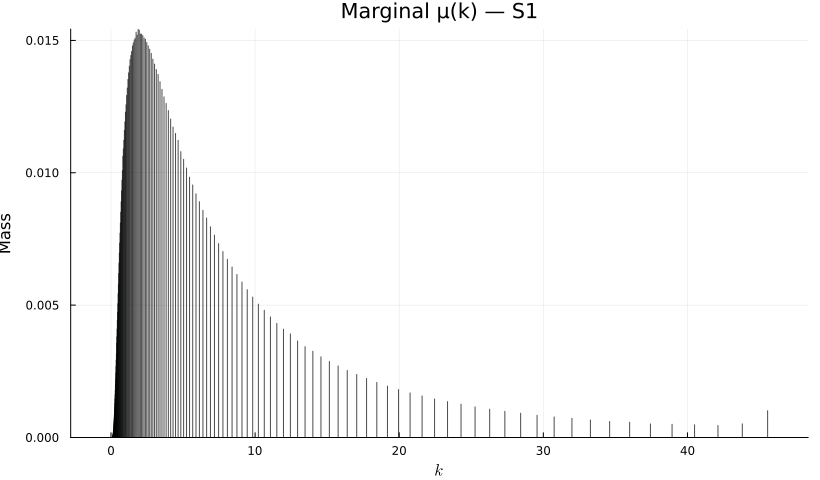
\includegraphics[width=\textwidth]{fig/s1_marginal_k.png}
        \caption{Marginal Capital for $z$ levels in Case 1}
        \label{fig:s1_marginal_k}
    \end{figure}
\end{minipage}

\vspace{\baselineskip}

The histogram depicts a t-Student like distribution of investment rates centered around 0.
Notably, we see that positive adjustments are much more preferred in this parameterization.
The marginal distributrion of capital also shows a intuitive pattern where higher k recieve decreaseing probability mass.


\subsection{Case 2: Fixed Costs}\label{subsec:fixed_costs}

Case 2 introduces fixed costs to the model with $F=0.05$ while keeping reversibility intact with $\rho_s = 1.0$.
As per the moment heatmap in Figure~\ref{fig:moment_heatmap}, we would expect an increase in inaction compared to the first case.

\vspace{\baselineskip}
\begin{minipage}{0.45\textwidth}
    \begin{figure}[H]    
        \centering
        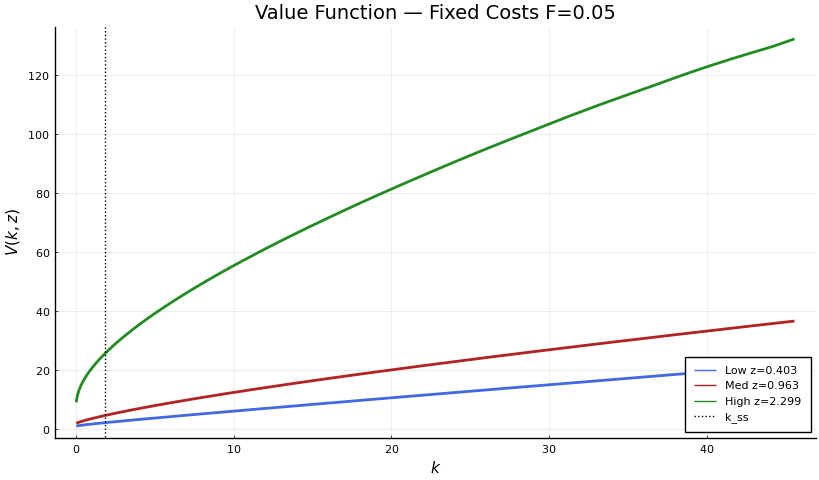
\includegraphics[width=0.8\textwidth]{fig/s2_value.png}
        \caption{Value Function for $z$ levels in Case 2}
        \label{fig:s2_value}
    \end{figure}
\end{minipage}\hfill
\begin{minipage}{0.45\textwidth}
    \begin{figure}[H]
        \centering
        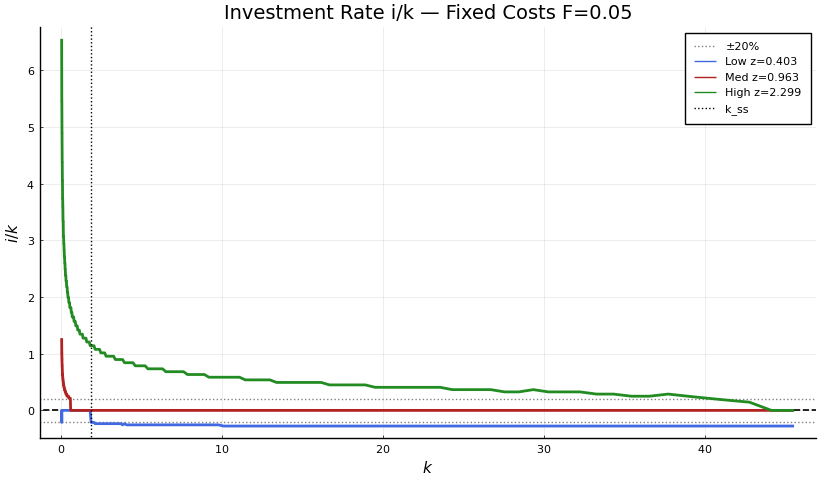
\includegraphics[width=0.8\textwidth]{fig/s2_ir.png}
        \caption{Investment Rates for $z$ levels in Case 2}
        \label{fig:s2_ir}
    \end{figure}
\end{minipage}
\vspace{\baselineskip}

The value function in Figure~\ref{fig:s2_value} shows a similar pattern to the first case; however, we see that the computed values are slightly lower in comparison.
This is perfectly sensible as the presence of added costs to the model.
The investment rates in Figure~\ref{fig:s2_ir} tell a more interesting story.
Looking at the plot, we observe that low productivity firms overwhelmingly choose to disinvest while medium firms remain inactive. 
High productivity firms follow a relatively similar path to their first case counterparts.

\vspace{\baselineskip}
\begin{minipage}{0.45\textwidth}
    \begin{figure}[H]
        \centering
        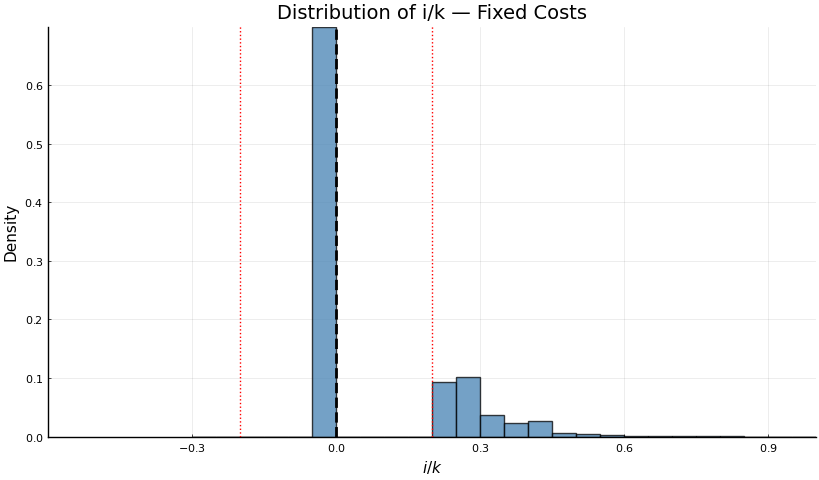
\includegraphics[width=\textwidth]{fig/s2_ir_hist.png}
        \caption{Histogram of Investment Rates for $z$ levels in Case 2}
        \label{fig:s2_hist}
    \end{figure}
\end{minipage}\hfill
\begin{minipage}{0.45\textwidth}
    \begin{figure}[H]
        \centering
        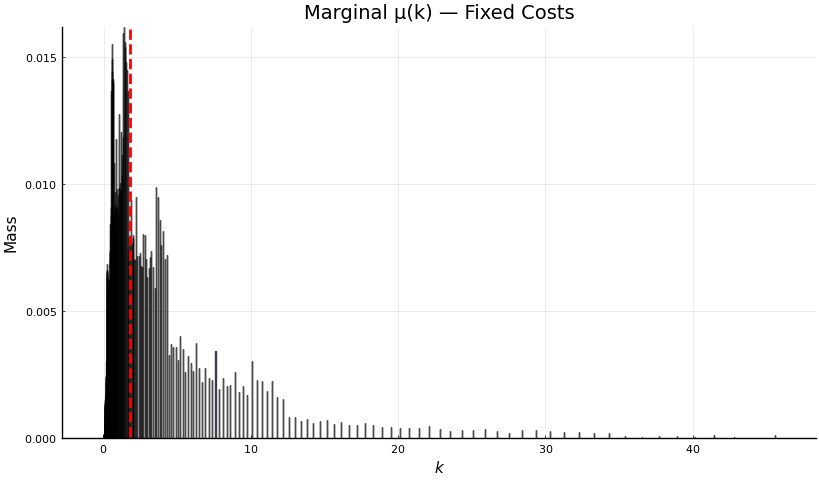
\includegraphics[width=\textwidth]{fig/s2_marginal_k.png}
        \caption{Marginal Capital for $z$ levels in Case 2}
        \label{fig:s2_marginal_k}
    \end{figure}
\end{minipage}
\vspace{\baselineskip}

While the marginal distribution of capital in Figure~\ref{fig:s2_marginal_k} is relatively consistent with the previous case, we see the suspected increase in inactivity with a comparatively massive peak around 0.
Also, it's important to note that the bin around 0 on the negative side, including the disinvestment we observe with low productivity firms.

\subsection{Case 3: Fixed Costs + Irreversibility}\label{subsec:fixed_irreversible}
The final case introduces irreversibility to the model with $\rho_s = 0.5$ and keeps the fixed costs from the previous case.
Again referring to the moment heatmap in Figure~\ref{fig:moment_heatmap}, we expect an increase in inaction similar to the previous case and a decrease in negative investment.

\vspace{\baselineskip}
\begin{minipage}{0.45\textwidth}
    \begin{figure}[H]    
        \centering
        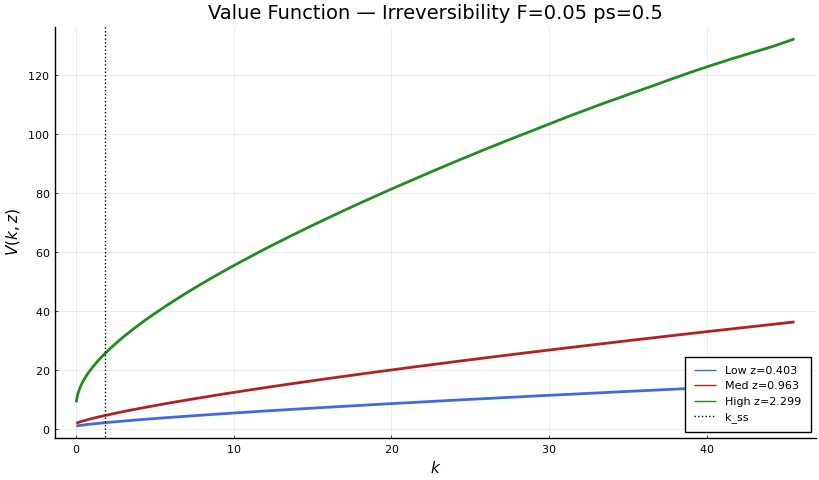
\includegraphics[width=0.8\textwidth]{fig/s3_value.png}
        \caption{Value Function for $z$ levels in Case 3}
        \label{fig:s3_value}
    \end{figure}
\end{minipage}\hfill
\begin{minipage}{0.45\textwidth}
    \begin{figure}[H]
        \centering
        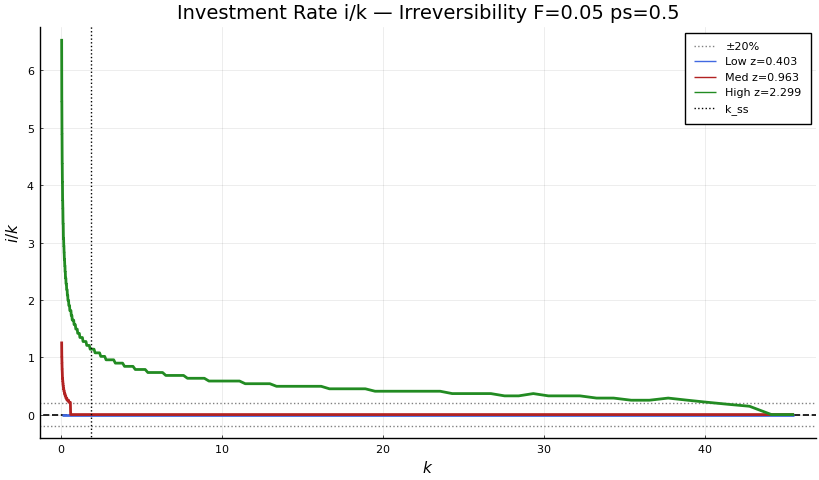
\includegraphics[width=0.8\textwidth]{fig/s3_ir.png}
        \caption{Investment Rates for $z$ levels in Case 3}
        \label{fig:s3_ir}
    \end{figure}
\end{minipage}
\vspace{\baselineskip}

We see that the value function in Figure~\ref{fig:s3_value} is near undifferentiable from that of case 2. We can reason that this is likely caused by inactivity being already very high in case 2 and the addition of irreversibility does not change the value function much.
The investment rates in Figure~\ref{fig:s3_ir} shows a similar picture with a key difference compared to case 2.
We observe that no class of firms choose to disinvest, which is consistent with the intuition that irreversibility should discourage negative adjustments.

\vspace{\baselineskip}
\begin{minipage}{0.45\textwidth}
    \begin{figure}[H]
        \centering
        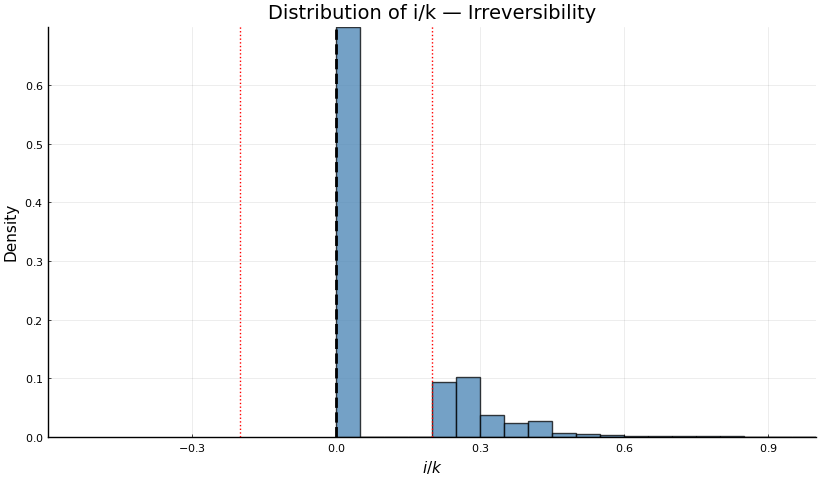
\includegraphics[width=\textwidth]{fig/s3_ir_hist.png}
        \caption{Histogram of Investment Rates for $z$ levels in Case 3}
        \label{fig:s3_hist}
    \end{figure}
\end{minipage}\hfill
\begin{minipage}{0.45\textwidth}
    \begin{figure}[H]
        \centering
        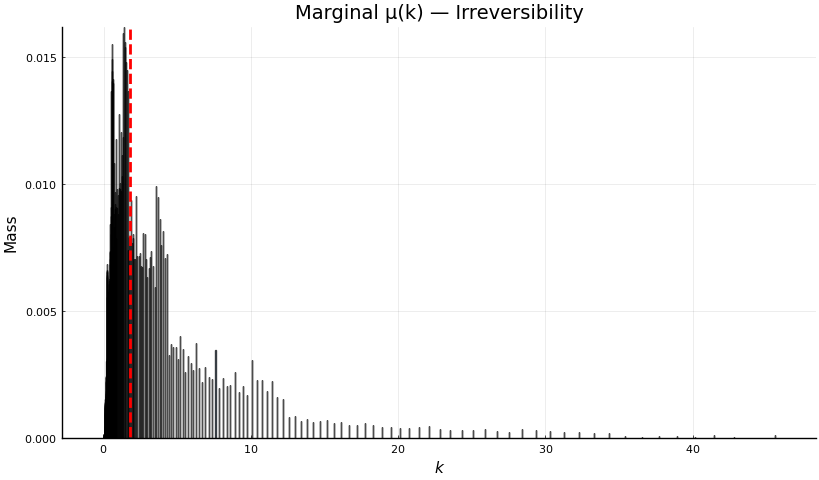
\includegraphics[width=\textwidth]{fig/s3_marginal_k.png}
        \caption{Marginal Capital for $z$ levels in Case 3}
        \label{fig:s3_marginal_k}
    \end{figure}
\end{minipage}
\vspace{\baselineskip}

The histogram of investment rates in Figure~\ref{fig:s3_hist} is basically identical to case 2 with again a single key difference.
Due to the lack of disinvestment, we see that the spike on 0 is positioned towards the positive side of the distribution.
However, the marginal distribution of capital shows no identifiable difference between the two cases.

\subsection{MoM Estimation of Model Parameters}
After analyzing the cases, we move onto estimating the parameters using MoM against the given data.
We apply estimation via moment computations from the stationary distributions and do not use Monte-Carlo or otherwise simulate data.

Applying said methodology, we obtain the following parameter estimates:

\begin{figure}[H]
    \begin{align}
        \hat{F} &= 0.00001 \\
        \hat{\rho}_s &= 0.9978 \\
        \hat{\gamma}_{adj} &= 2.9703
    \end{align}
    \caption{Estimated Parameters}
\end{figure}
\noindent The moments obtained from the estimated parameters are compared to the cases as follows:
\begin{table}[H]
    \begin{tabular}{l c c c c c}
        
            \toprule
            Moment & LRD Target & Case 1 & Case 2 & Case 3 & Final Calibration \\
            \midrule
            Avg. Investment Rate (\%) & 12.2 & 8.63 & 8.96 & 8.96 & 8.42\\
            Inaction Rate (\%)$^*$ & 8.1 & 11.31 & 69.86 & 69.9 & 9.32 \\
            Fraction Negative(\%) & 10.4 & 21.88 & 0.02 & 0.0 & 16.14\\
            Positive Spike Rate(\%)$^*$ & 18.0 & 15.6 & 30.12 & 30.1 & 9.52 \\
            Negative Spike Rate(\%)$^*$ & 1.4 & 0.0 & 0.02 & 0.0 & 0.0 \\
            \bottomrule
    \end{tabular}

    {\noindent\RaggedRight\footnotesize $^*$ Moments that are targeted in the objective function}
    \caption{Estimated moments and moments from cases}
\end{table}

We see that the estimates are rather inaccurate in matching the target moments.
This could partly be attributed to our difficulty in getting average investment rates to adjust over 9\% and the fact that we could not estimate non-zero negative spikes even when targeting it by itself.
However, we picked our target moments to each correspond to (and contribute information related to) a specific parameter.
Specifically, we chose inaction rates as a target to capture the fixed costs, while positive spike rates were chosen to capture the positive effect of $\gamma_{adj}$ on investment rates.
Similarly, we chose negative spike rates to capture the negative effect of the presence of irreversibility. 